\documentclass{beamer}

\usepackage{txfonts}
\usepackage{hyperref}
\usepackage{fancybox}
\usepackage{xfrac}
\usepackage{cancel}


\newcommand{\heart}{\ensuremath\heartsuit}

\usepackage{mathtools,amssymb}
\newcommand{\myarrow}{\scalebox{2}[2]{$\mathclap{\curvearrowleft}\mkern2.2mu
                                                 \mathclap{\curvearrowright}$}}

\DeclareMathOperator{\Bin}{\mathrm{Bin}}

\hypersetup{colorlinks=false,linkbordercolor=red,linkcolor=green,pdfborderstyle={/S/U/W 1}}

\addtobeamertemplate{navigation symbols}{}{ \hspace{1em}    \usebeamerfont{footline}%
    \insertframenumber / \inserttotalframenumber}

\geometry{papersize={15cm,13cm}}
\usepackage{lipsum}

\makeatletter
\newenvironment<>{contdproof}[1][\proofname]{%
    \par
    \def\insertproofname{#1\@addpunct{.}}%
    \usebeamertemplate{proof begin}#2}
  {\usebeamertemplate{proof end}}
\makeatother


\setbeamertemplate{theorems}[numbered]

\newtheorem*{nonumdefinition}{Definition}
\newtheorem*{nonumproblem}{Problem}
\newtheorem*{nonumlemma}{Lemma}
\newtheorem*{nonumtheorem}{Theorem}
\newtheorem*{nonumproof}{Proof}
\newtheorem*{nonumremark}{Remark}
\newtheorem*{answer}{Answer}
\newtheorem*{nonumremarks}{Remarks}
\newtheorem*{nonumexamples}{Examples}
\newtheorem*{nonumsolution}{Solution}
\newtheorem*{nonumexample}{Example}
\newtheorem*{nonumproposition}{Proposition}

\newtheorem{remark}{Remark}
\newtheorem{exam}{Example}




\theoremstyle{alphtheorem}
\newtheorem{alphtheorem}{Theorem}
\renewcommand{\thealphtheorem}{\Alph{alphtheorem}}
\renewcommand{\thesection}{\arabic{section}}



\usepackage{tikz}
\newcommand*\mycirc[1]{%
  \tikz[baseline=(C.base)]\node[draw,circle,inner sep=.7pt](C) {#1};\:
}

\newcommand\myheading[1]{%
  \par\bigskip
  {\color{blue}{\large #1}}\par\smallskip}

%\usetheme{Warsaw}
%\usetheme{Berkeley} %sample 1

\usetheme{Berlin} % sample 2
%\usetheme{AnnArbor} % sample 3

\let\otp\titlepage
\renewcommand{\titlepage}{\otp\addtocounter{framenumber}{-1}}

\title{Lecture 25: Stat 400, Lecture 25 Sampling from $N(\mu, \sigma^2)$ and the CLT}
\author{}
\date{}

\begin{document}
\begin{frame}

\medskip
{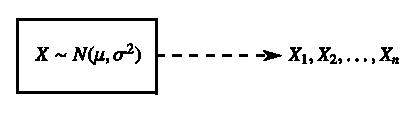
\includegraphics{figure/art25(1).eps}}

\smallskip

Suppose $X_1, X_2, \ldots, X_n$ is a random sample from a normal population. We have seen that we should use the \underline{sample} mean $\overline{X}$ to estimate the population mean $\mu$ and the \underline{sample} variance $S^2$ to estimate the population variance $\sigma^2$.
\end{frame}

\begin{frame}
$\overline{X}$ and $S^2$ are random variables. 

\underline{$\$$ 64,000 question}

How are $\overline{X}$ and $S^2$ distributed ? The answer is given by the following considerations 

Any linear combination of Independent normal random variables is again normal so $\overline{X}$ is normal. Since $E(\overline{X}) = \mu$ and $V(\overline{X}) = \dfrac{\sigma^2}{n}$ we have
$$
\overline{X} \sim N \left(\mu , \dfrac{\sigma^2}{n} \right)
$$
\end{frame}

\begin{frame}
Suppose $Z$, $Z_2,\ldots, Z_n$ are independent standard normal random variables. Then 
\begin{equation*}
Z^2_1 + \ldots + Z^2_b \sim \chi^2(n) \tag{$\ast$}
\end{equation*}

Chi-squared with $n$ degrees of 
$$
\text{Now ~~~} \qquad  Z_i = \frac{X_i - \mu}{\sigma} \sim N (0,1)
$$
So
$$
\sum\limits^n_{i=1} \left(\frac{X_i-\mu}{\sigma} \right)^2 = \frac{1}{\sigma^2} \sum\limits^n_{i=1} (X_i - \mu)^2 \sim \chi^2 (n)
$$

Now replace $\mu$ by its estimation $\overline{X}$ Rule of thumb - \textit{every time you replace a quantity by its estimator you lose one degree of freedom in the chi-squared distribution}
\end{frame}

\begin{frame}
So by the ``rule of thumb''
$$
Y = \frac{1}{\sigma^2} \sum\limits^n_{i=1} (X_i - \overline{X})^2 \sim \chi^2 (n-1)
$$
Now $S^2 = \dfrac{1}{n-1} \sum\limits^n_{i=1} (X_i - \overline{X})^2$

So $Y = \dfrac{n-1}{\sigma^2} S^2$ and we  obtain the critical
\begin{equation*}
\frac{n-1}{\sigma^2} S^2 \sigma \chi^2 (n-1) \tag{$\ast\ast$}
\end{equation*}

\begin{nonumremark}
This isn't a proof because we used ``the rule of thumb'' but the result is true
\end{nonumremark}
\end{frame}

\begin{frame}
\underline{Bottom Line}

\begin{nonumtheorem}
Let $X_1, X_2, \ldots, X_n$ be a random Sample from a normal population with mean $\mu$ and variance $\sigma^2$. Then 
\begin{itemize}
\item[(i)] $\overline{X} \sim N \left(\mu, \dfrac{\sigma^2}{n} \right)$
 
\item[(ii)] $\dfrac{n-1}{\sigma^2} S^2 \sim \chi^2 (n-1)$

\item[(iii)] $\overline{X}$ and $S^2$ are independent.
\end{itemize}

The above statement is on exact  statement but if we take a large sample $(n>30)$ from \underline{any} population with mean $\mu$ and variance $\sigma^2$ we may assume
\end{nonumtheorem}
\end{frame}
\begin{frame}
\begin{nonumtheorem}[Cont.]
to a good approximation that the population has $N(\mu, \sigma^2)$ distribution and we have by CLT
\end{nonumtheorem}

\begin{nonumtheorem}
If $X_1, X_2, \ldots, X_n$ is a \underline{large} $(n > 30)$ random sample from \underline{any} population with mean $\mu$ and variance $\sigma^2$ then 
\begin{itemize}
\item[(i)] $\overline{X} \approx N (\mu , \dfrac{\sigma^2}{n})$

\item[(ii)] $S^2 \approx \chi^2 (n-1)$

\item[(iii)] $\overline{X}$ and $S^2$ are \underline{approximately} independent. (then are not independent unless the population is normal.)
\end{itemize}
\end{nonumtheorem}
\end{frame}

\end{document}




